\iffalse
\documentclass[12pt]{article}
\usepackage{graphicx}
%\documentclass[journal,12pt,twocolumn]{IEEEtran}
\usepackage[none]{hyphenat}
\usepackage{graphicx}
\usepackage{listings}
\usepackage[english]{babel}
\usepackage{graphicx}
\usepackage{caption} 
\usepackage{hyperref}
\usepackage{booktabs}
\usepackage{commath}
\usepackage{gensymb}
\usepackage{array}
\usepackage{amsmath}   % for having text in math mode
\usepackage{listings}
\lstset{
  frame=single,
  breaklines=true
}
  
%Following 2 lines were added to remove the blank page at the beginning
\usepackage{atbegshi}% http://ctan.org/pkg/atbegshi
\AtBeginDocument{\AtBeginShipoutNext{\AtBeginShipoutDiscard}}
%


%New macro definitions
\newcommand{\mydet}[1]{\ensuremath{\begin{vmatrix}#1\end{vmatrix}}}
\providecommand{\brak}[1]{\ensuremath{\left(#1\right)}}
\providecommand{\norm}[1]{\left\lVert#1\right\rVert}
\newcommand{\solution}{\noindent \textbf{Solution: }}
\newcommand{\myvec}[1]{\ensuremath{\begin{pmatrix}#1\end{pmatrix}}}
\let\vec\mathbf
\begin{document}
\begin{center}
\title{\textbf{Circles}}
\date{\vspace{-5ex}} %Not to print date automatically
\maketitle
\end{center}
\setcounter{page}{1}
\section{11$^{th}$ Maths - Exercise 11.1.8}

\begin{enumerate}
\item Find the centre and radius of the given circle $x^2+y^2-8x+10y-12=0$
\section{Solution}
\fi
From the given informtion,
\begin{align}
 \vec{u}=\myvec{-4\\5},\,
 f&=-12\\
\implies \vec{c}&=\myvec{4 \\ -5},\\
	r=\sqrt{\norm{\vec{u}}^2-f}
&=\sqrt{53}
\end{align}
See Fig. 
\ref{fig:chapters/11/11/1/8/Fig1}.
\begin{figure}[!h]
	\begin{center} 
	   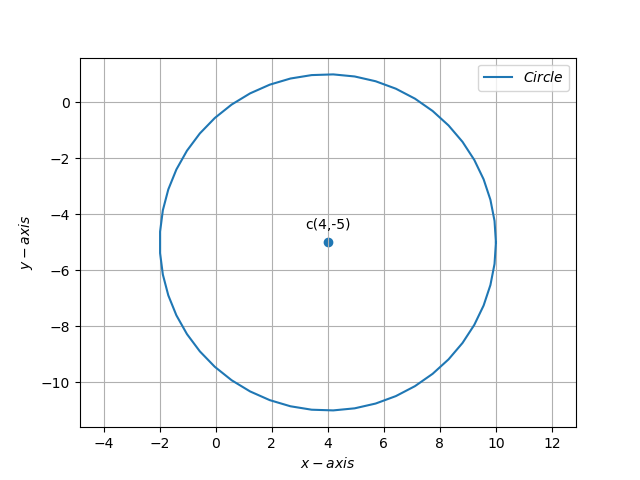
\includegraphics[width=\columnwidth]{chapters/11/11/1/8/figs/11.1.8.png}
	\end{center}
\caption{}
\label{fig:chapters/11/11/1/8/Fig1}
\end{figure}
